\chapter{System Design} \label{chapter:ch3_system_design}

Chapter~\ref{chapter:ch2_analysis} motivated a modular architecture with explicit interfaces, so that sensing, UI, robot backends, and task logic can be exchanged without rewriting the whole system. This chapter describes the design of this modular system and the main interfaces that enable communication between its components.

\section{System at a glance} \label{sec:ch3_overview}

\begin{figure}
  \centering
  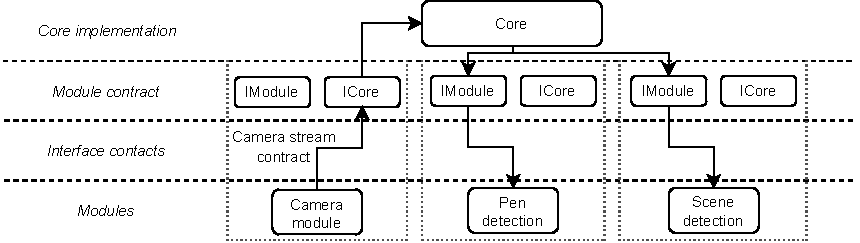
\includegraphics[width=\textwidth]{img/ch3_system_design/four_parts.pdf}
  \caption{Conceptual separation of contracts and implementations. The module contract defines how modules interact with the runtime core (lifecycle + message exchange). Interface contracts specify domain message semantics (e.g., camera stream, pen pose, scene detection) on top of the module contract. Concrete modules implement these contracts, while the core provides one concrete hosting and routing implementation.}
  \label{fig:ch3_four_parts}
\end{figure}

The system is organized into four conceptual parts, shown in \autoref{fig:ch3_four_parts}. This separation helps to keep the design modular: stable contracts are defined once, while concrete implementations can be replaced as the system evolves.

\begin{enumerate}[label=(\arabic*), itemsep=0.3em]
    \item \textbf{Module contract.}
    This part defines \emph{what a module is} and how modules interact, without assuming a specific runtime implementation. It does so by specifying the module and core contracts.
    It specifies the communication primitives (publish/subscribe and request/response), message structure (small headers with optional shared blobs for large data), channel declaration, channel mapping, module lifecycle and abstract core API.
    All module code depends only on this contract.

    \item \textbf{Core implementation.}
    The core is the concrete runtime that \emph{implements} the module contract.
    It is responsible for loading modules, instantiating them, applying the channel mapping, routing messages, scheduling message processing, and managing shared memory for large payloads.
    Different core implementations are possible in principle (threads, processes, distributed), while still keeping the same module contract.

    \item \textbf{Interface contracts.}
    On top of the generic module communication, we define standard interfaces for our application domain (e.g., robot control, scene data, camera image) and for UI interaction (e.g., activation, use case execution, 3D visualization). These interfaces define \emph{what} messages mean and what behavior other modules can rely on, independent of a specific module's implementation of the required functionality.

    \item \textbf{Modules.}
    Finally, the concrete functionality is implemented as modules: camera acquisition, calibration, 6D pen input, scene detection, use cases, and robot execution. UI itself is also implemented as a module, since it is just another component that interacts with others through the defined interfaces.
    These modules use the standard interfaces and are hosted by the runtime core.
    As long as the interfaces are respected, modules can be added, removed, or replaced with minimal impact on the rest of the system.
\end{enumerate}

In the remainder of this chapter, we describe these parts in the same order: first the module contract, then the concrete core implementation, and finally the interface contracts. Implementation details of the actual modules are covered in \autoref{chapter:ch4_implementation}.



\section{Module contract}

This section defines the \emph{module contract}: the core abstractions and communication rules that all modules and the runtime core must follow. The contract is independent of a concrete core implementation and provides a stable interface for developing modules.

\subsection{Roles and separation of responsibilities} \label{subsec:ch3_roles}

The contract separates responsibilities between modules and the core through two interfaces: \type{IModule} and \type{ICore}. Each module implements \type{IModule}, which defines its lifecycle, message handling entry points, serialization of module state, and other required methods. The core exposes \type{ICore}, which provides services to modules, including message routing, shared-memory allocation for large payloads, and system management operations (module discovery, instantiation, save/load, etc.).

As shown in \autoref{fig:ch3_four_parts}, modules do not communicate directly. All interaction goes through the core, which routes messages between modules according to an explicit channel mapping. When a module publishes data or sends a request/response, it calls the corresponding method on \type{ICore}; the core then delivers the message to the mapped recipient(s).

On the receiving side, the core enqueues the incoming message and later invokes the appropriate \type{IModule} callback from a core-managed worker thread. The contract therefore assumes concurrent execution: multiple worker threads may call into the same module instance at the same time (same or different channels, or overlapping message and request handling). Modules must treat these callbacks as multi-threaded entry points and synchronize access to their internal state accordingly. The concrete queueing and worker configuration is part of the module declaration and is described next.

\subsection{Module description contract}

\begin{figure}
  \centering
  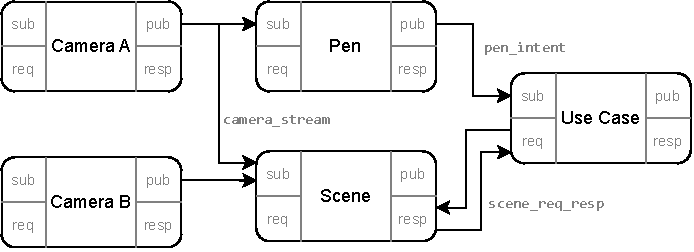
\includegraphics[width=\textwidth]{img/ch3_system_design/channel_mapping.pdf}
  \caption[Example of a channel mapping]{Example of a channel mapping; \type{Camera A} and \type{Camera B} both produce \type{camera_stream} messages; \type{Pen} consumes \type{camera_stream} messages from \type{Camera A} and produces \type{pen_intent} messages. \type{Scene} consumes \type{camera_stream} messages from both \type{Camera A} and \type{Camera B} and contains a response producer channel for \type{scene_req_resp} messages. \type{Use Case} consumes \type{pen_intent} messages from \type{Pen} and sends \type{scene_req_resp} requests to \type{Scene} and consumes the corresponding responses.}
  \label{fig:ch3_channel_mapping}
\end{figure}

To support different communication patterns, the contract provides two complementary primitives: publish/subscribe for streams and request/response for on-demand queries. Publish/subscribe is used for continuously produced data such as camera frames, while request/response is used when work should happen only when requested (e.g., a scene module performs detection only after receiving a request and returns detected objects). Modules therefore declare their inputs (consumers: subscribe or request) and outputs (producers: publish or response). Each channel is tagged by a \emph{channel type identifier} (string) that specifies the message type. An example wiring is shown in \autoref{fig:ch3_channel_mapping}.

Each module describes itself using a \type{ModuleInfo} structure, which includes:
\begin{itemize}
    \item \textbf{Module identifiers and UI text:} module type identifier, display name, and description,
    \item \textbf{Channel declarations:} lists of publish producers, response producers, subscribe consumers, and request consumers,
    \item \textbf{Instantiation policy:} auto-create flag,
    \item \textbf{Concurrency configuration:} number of worker threads (described below).
\end{itemize}

Channel declarations specify what the module can produce and what it requires as input. Importantly, communication is not a broadcast by default: connections are \emph{directed} between specific producer and consumer channels. The channel type identifier defines compatibility (message type), but the actual wiring is provided at module instantiation time via a channel mapping. The mapping selects, for each consumer channel, which producer channel(s) it is connected to (by specifying producer module and channel IDs). This enables flexible configurations---for example, in \autoref{fig:ch3_channel_mapping} the \type{Pen} module subscribes only to \type{Camera A} even though multiple cameras publish \type{camera_stream}.

As noted in \autoref{subsec:ch3_roles}, message processing is executed by core-managed worker threads. Each module specifies how many worker threads it requires, allowing it to process multiple messages, requests or responses concurrently. Worker threads are created per module and are divided into two classes: \emph{prioritized} and \emph{regular}. Prioritized workers handle channels marked as prioritized; regular workers handle the remaining channels. This mechanism is crucial for UI responsiveness, because it allows latency-sensitive UI traffic to be processed in parallel with heavy computation (e.g., camera processing for pen tracking).

Finally, the auto-create flag marks modules that are instantiated automatically when the system starts (e.g., the UI module). Auto-created modules cannot depend on a manually provided channel mapping. In this thesis, we therefore restrict auto-created modules to \emph{AUTO\_ALL} consumer channels: they may declare inputs, but only in a form that can be wired automatically to all currently available producers of the given type (see \autoref{subsec:ch3_channel_contract}).

\subsection{Channel contract} \label{subsec:ch3_channel_contract}

In the previous section, we described how modules declare their inputs and outputs using channels. In this section, we define the channel structures and the wiring constraints in more detail.

Channel definitions are provided \emph{per module} as part of its \type{ModuleInfo}: they describe the module's channel \emph{endpoints} (what it can produce and what it can consume). Concrete \emph{connections} between endpoints are created by the core when a module is instantiated, by binding consumer endpoints to selected producer endpoints according to the provided channel mapping.

There are two kinds of channels: producer channels (described by \type{Producer} structure) and consumer channels (described by \type{Consumer} structure).

A \type{Producer} contains:
\begin{itemize}
    \item channel type identifier (e.g., \type{camera_stream}, \type{scene_req_resp}),
    \item user-facing channel name and description (used for UI visualization),
    \item prioritized flag,
    \item message queue capacity (maximum number of pending items on the receiver side).
\end{itemize}

Prioritization on the producer side is only relevant for response producers: if a response producer is prioritized, the corresponding request is processed by a prioritized worker thread in the receiving module.

We define message queue capacity to bound the amount of pending work at the receiver. If messages or requests arrive faster than the module can process them, the queue capacity prevents unbounded buffering; the module can then decide how to handle overload (drop, replace, etc.), described in \autoref{subsec:ch3_message_lifecycle}.

A \type{Consumer} contains:
\begin{itemize}
    \item channel type identifier, name, description, prioritized flag, and message queue capacity (same meaning as in \type{Producer}),
    \item count policy (\type{single}, \type{range} or \type{auto_all}); specifies how many producer endpoints of the same type must be bound to this consumer endpoint when the module is instantiated,
    \item min/max bounds (used only for the \type{range} policy).
\end{itemize}

When \type{ICore::addModule} is called, the core validates that the provided channel mapping satisfies these constraints (type match and required cardinality bounds); otherwise the module instantiation fails.

Prioritization on the consumer side applies to both subscribe and request channels. If a subscribe consumer is prioritized, incoming messages are processed by a prioritized worker thread. If a request consumer is prioritized, the corresponding response is processed by a prioritized worker thread.

The count policy expresses wiring requirements. With \type{single}, exactly one producer endpoint of the given type must be connected. With \type{range}, the consumer requires between \type{min} and \type{max} connected producer endpoints (inclusive). With \type{auto_all}, the consumer is wired automatically to all currently available producer endpoints of the given type, which is primarily used for auto-created modules that cannot receive an explicit mapping. For example, the UI module can subscribe to all available \type{camera_stream} producers via an \type{auto_all} subscribe consumer, combining the convenience of broadcast with the explicit wiring model used elsewhere.

\subsection{Message structure: header and optional shared blobs}

The message model is designed to efficiently handle both small control messages and large data payloads. All messages are represented by the \type{MessageHeader} structure, which is used uniformly for publish/subscribe as well as request/response communication.

The header contains:
\begin{itemize}
    \item \textbf{Small copied payload} given by a data pointer and length. This part is intended for small, trivially copyable control data (e.g., pen intent, state updates) and is copied from the producer to each consumer.
    \item \textbf{Optional blob array} (pointer + count), representing one or more shared payloads used for large data (e.g., images, point clouds, serialized structures) that should not be copied repeatedly.
    \item \textbf{Request/response metadata:} \type{id_} to match requests with responses and a \type{success_} flag indicating whether the request was processed successfully at the communication layer.
    \item \textbf{Timestamp} (\type{timestamp_ns_}) for tracing and ordering.
\end{itemize}

In practice, most messages consist only of the small copied payload. When large data needs to be transmitted, the message includes one or more blobs. A producer allocates a blob, writes the payload into it, and sends a message that references the blob. Consumers can then read the payload directly and may forward the same blob further (e.g., camera $\rightarrow$ calibration $\rightarrow$ pen tracking) without copying the underlying data.

\subsection{Shared payload ownership and allocator contract}

Large payloads are represented by \type{SharedDataBlob}, which acts as a handle to core-managed shared data (\type{ISharedData}). Modules never free raw memory directly. Instead, they only copy, store, and pass \type{SharedDataBlob} handles; the underlying shared memory is released automatically once the last handle is destroyed.

Blobs are allocated through core-provided allocators (\type{IAllocator}). A module can request an allocator via \type{ICore::createDynamicAllocator()} or \type{ICore::createBufferAllocator(slot_size, slot_count)} and then allocate blobs using \type{IAllocator::allocate()} (or helper methods such as \type{allocateFromData}). We distinguish two allocator types at the contract level:
\begin{itemize}
    \item \textbf{Dynamic allocator:} supports variable allocation sizes (suitable for irregular payloads such as scene snapshots) at the cost of relying on system allocations for each request.
    \item \textbf{Buffer allocator:} preallocates a fixed number of equally-sized slots (suitable for streaming payloads with known bounds, such as camera frames), requiring a known maximum size in advance and offering only a limited number of slots.
\end{itemize}

Allocator and blob lifetime are owned by the core to ensure consistent memory management across modules and to allow safe sharing between independently developed components. Modules are expected to delete allocators they no longer need using \type{ICore::deleteAllocator}. In this thesis, allocator cleanup is handled by the common \type{BaseModule} helper (\autoref{subsec:ch3_basemodule}) so that module implementations do not need to manage allocator lifetimes manually.


\subsection{Communication primitives (semantics only)}

This subsection describes the runtime semantics of the two communication primitives. Channel declaration and mapping rules are defined by \type{ModuleInfo} and the channel contract (\autoref{subsec:ch3_channel_contract}). All channels in this sections contain a module identifier and a channel identifier (index into the module's channel list --- publish producer list for publishing message, request consumer list or response producer list for request/response logic), which together uniquely identify the channel endpoint in the system.

\textbf{Publish/subscribe} is used for streams and events. A module publishes a message by calling \type{ICore::sendMessage(source_channel, message)} with \type{source_channel} identifying its producer channel. The core routes the message to all subscribe consumers that are connected to this producer by the current mapping. Delivery is best-effort and may be affected by the receiver's ingress and queueing policy (\autoref{subsec:ch3_message_lifecycle}).

\textbf{Request/response} is used for directed on-demand interactions. The requester calls \type{ICore::sendRequest(source_channel, target_channel, message)} and specifies both its local request consumer channel (\type{source_channel}) and the \emph{concrete} target response producer channel (\type{target_channel}) it is requesting from. The core delivers the request to the receiver by invoking \type{IModule::processRequest(response_producer_id, source_channel, message)}. The receiver returns the response payload as \type{ResponseData}; the core (or the module hosting wrapper) then sends exactly one response back to the requester via \type{ICore::sendResponse(source_channel, target_channel, message)} with the response producer as \type{source_channel} and the original request consumer as \type{target_channel}. This design prevents modules from silently ``forgetting'' a request and ensures a well-defined one-request/one-response flow at the transport level.

\textbf{Synchronous vs asynchronous aspects.} On the receiver side, \type{IModule::processRequest} produces the response data synchronously (as a return value). From the requester perspective, request/response is still asynchronous: the response is delivered later via \type{IModule::processResponse} and must not be assumed to arrive immediately or on the same thread.

\textbf{Success and failure.} The field \type{MessageHeader.success_} represents transport-level outcome (e.g., request dropped or rejected, invalid routing). Domain-level success (e.g., detection failed) is encoded in the payload and is specific to each channel type.


\subsection{Message delivery flow} \label{subsec:ch3_message_lifecycle}

Message delivery follows the same contract-level steps for publish/subscribe as well as request/response:

\begin{enumerate}
    \item The sender calls \type{ICore::sendMessage} / \type{ICore::sendRequest} / \type{ICore::sendResponse} and provides the source channel identifier (and a target identifier for request/response).
    \item The core determines the destination module(s) and consumer channel(s):
    \begin{itemize}
        \item \textbf{Publish/subscribe:} the core resolves routing using the current channel mapping (i.e., the producer is routed to all mapped subscribe consumers).
        \item \textbf{Request/response:} the destination is given explicitly by \type{target_channel}. The core validates that the target endpoint is compatible with the sender's mapping policy (e.g., within \type{SINGLE}/\type{RANGE}; \type{AUTO_ALL} does not require a specific mapping check).
    \end{itemize}
    \item For each destination consumer, the core calls the receiver's ingress decision point \type{IModule::onIngress} and provides the message header and the current queue status.
    \item If the message is rejected (or must be dropped due to capacity), it is not delivered. For requests, the transport-level failure is reported back to the requester as a failed response (\type{success_ = false}).
    \item If accepted, the core enqueues the message for processing. The enqueued item includes an owned copy of the small payload buffer and a copied list of \type{SharedDataBlob} handles. The underlying shared payload memory referenced by blobs is not copied.
    \item The core invokes the corresponding module callback from a core-managed worker thread: \type{IModule::processMessage}, \type{IModule::processRequest}, or \type{IModule::processResponse}.
    \item For requests, the receiver returns \type{ResponseData} from \type{IModule::processRequest}. The core (or the hosting wrapper) constructs exactly one response message, preserves the request \type{id_}, and sends it back to the requester, where it is delivered by the same process described here via \type{IModule::processResponse}.
\end{enumerate}

The ingress decision point \type{IModule::onIngress} is a required part of the contract and must be \emph{non-blocking}. It is executed on the core's delivery path and is therefore intended only for a fast admission-control decision under load. The core passes a \type{QueueStatus} describing whether the destination queue has available capacity. The module may then return an \type{IngressDecision} to either accept, drop, or (when allowed) drop/replace queued work (e.g., keep only the latest frame for a video stream). If the queue is already in \type{QUEUE_FULL} (queue is full, processing started on all messages, but did not finish yet), all decisions are effectively treated as drop.

The concrete scheduling mechanism (queues, worker pools, and prioritization) is part of the core implementation and is described in \autoref{sec:ch3_core}.



\subsection{Reflection and orchestration contract} \label{subsec:ch3_reflection_orchestration}

Besides message passing, the contract exposes a small \emph{reflection and orchestration} API intended mainly for UI and other controller-style modules. Its purpose is to allow a module to (i) discover what module types exist, (ii) inspect which module instances are currently running and how they are wired, and (iii) create, remove, save, and restore module graphs. This functionality is provided through the \type{ICoreControl} part of \type{ICore}.

\textbf{Loaded module catalog (module types).}
The core exposes a catalog of all module \emph{types} available in the runtime (e.g., discovered plugins). The pair \type{getLoadedModulesCount()} and \type{getLoadedModulesInfo(loaded_module_id)} allows querying each type's immutable \type{ModuleInfo} (declared channels, display metadata, auto-create flag, worker configuration, etc.). UI uses this catalog to present the user with a ``palette'' of modules that can be instantiated.

\textbf{Running module instances (created modules).}
While the loaded catalog lists available types, the runtime also maintains a set of created \emph{instances}. Each instance is assigned a \emph{monotonically increasing} running module identifier when created; identifiers are never reused. If an instance is later removed, its identifier becomes a tombstone that permanently refers to a non-existing module.

This contract is reflected in \type{RunningModuleInfo}, which contains an \type{exists_} flag and a reference to the instance's \type{ModuleInfo} (\type{module_info_}). The method \type{getRunningModulesCount()} returns the total number of identifiers issued over the lifetime of the core object (not the number of currently alive instances). Callers therefore iterate \type{running_module_id} from \type{0} to \type{getRunningModulesCount()-1} and query each entry via \type{getRunningModulesInfo(running_module_id)}, filtering out non-existing modules using \type{exists_}. Running module identifiers must not be assumed stable across program sessions or save/load.

\textbf{Wiring query (who is connected to whom).}
For each running module instance, \type{getRunningModulesChannelMap(running_module_id)} returns its current input wiring: for every subscribe and request consumer channel, the core provides the list of bound producer endpoints (\type{ChannelIdentifier} pairs identifying producer module and producer channel). This is the core reflection primitive needed to visualize or debug the module graph and to implement higher-level orchestration logic (e.g., configuration panels that depend on which sources are currently connected).

\textbf{Existing producers by channel type (discovery).}
For reflection and UI/orchestration, the core provides
\type{getExistingPublishChannelsByName(channel_type_identifier)} and
\type{getExistingResponseChannelsByName(channel_type_identifier)}.
These functions return the set of currently known producer endpoints (module ID + channel ID) for the given channel type identifier.

For \emph{SINGLE} and \emph{RANGE} request consumers, the requester typically does \emph{not} need discovery: the core provides the concrete mapped endpoints as part of \type{InputChannelMapInfo} during module creation, and the module uses those \type{ChannelIdentifier}s as request targets.
Discovery is primarily needed for \emph{AUTO\_ALL} request consumers, where the target set is not known at instantiation time (and therefore is not enumerated in \type{InputChannelMapInfo}).

\textbf{Mapping state change indicator.}
Because the running set and its wiring may change over time (modules created/removed), the core exposes \type{getModulesMappingStateId()}. The returned value is a monotonically increasing identifier that changes whenever the mapping topology changes (modules are added or removed). UI modules can use it as a cheap change detector to refresh cached views.

\textbf{Orchestration entry points (create/remove/dependencies).}
The contract allows a controller to create and remove modules dynamically. A new instance is created using \type{addModule(loaded_module_id, channel_map_info)}. The core validates the provided mapping against the declared channel contract (channel type identifiers and the consumer count policy such as single/range/auto-all) and rejects invalid wiring. Existing modules may be removed via \type{removeModuleById(running_module_id, recursive)}; when recursive removal is requested, the core may also remove dependent modules (as defined by the connection types), and \type{collectDependencies(running_module_id)} can be used to inspect this dependency set in advance.

\textbf{Persistence entry points (save/load).}
Finally, the contract provides \type{save()} and \type{load(data, size)} to persist and restore the \emph{program state} consisting of created module instances, their wiring, and optional per-module serialized state (as returned by module \type{save()} / \type{load()}). The binary format is owned by the core. Loading reconstructs the module graph from the loaded catalog; running and loaded module identifiers may change, and modules must not rely on ID stability across save/load. Allocators are not persisted; modules are expected to recreate any allocators they need after loading.



\subsection{Reflection and orchestration contract}

\xxx{or here serialization}

\subsection{Module lifecycle and implementer rules}

\xxx{thread start, stop methods; getModuleInfo; query\_capability; valid }
\xxx{mention thread requirements; no core calls in ctor / dtor; onIngress non-blocking; processing callbacks may be slow but must be safe under hosting concurrency; do not assume stable module IDs across save/load}
\xxx{see what is all multi-threaded and what is not}
\xxx{describe serialization}
\xxx{what must be provided in instanciation}
\xxx{module creation, what is given to the module (data path, module map etc.)}
\xxx{due to not knowing the runtime, modules are expected to *not* return any exceptions (exceptions crossing a dll/so boundary would be problematic)}
\xxx{Where do we mention c++, dll/so, windows/linux, etc.? in the core implementation section? Implementaion chapter?}
\xxx{thinking about it now, it would be much better/cleaner to do: The logic should be constructor (core-thread), initialize(core-requested, but separate thread after core finished creating; only after initialize finishes does it start processing messages?), teardown (core-thread, add-remove locked but general core not locked, modules can finish sending messages but must stop ASAP), destructor(core, full core locked, if modules send now it will cause undefined behavior). }

\subsection{BaseModule} \label{subsec:ch3_basemodule}

In this thesis, most modules inherit from \type{BaseModule}, a convenience helper that implements common boilerplate on top of \type{IModule}. In particular, it (i) fills required message metadata (\type{timestamp_ns_}, request \type{id_}, and transport \type{success_}), (ii) constructs correct \type{ChannelIdentifier} values using the module's runtime ID, (iii) provides RAII wrappers for core allocators, and (iv) exposes the construction-time parameters provided by the core (data path, logger, and the resolved input channel mapping) through simple helper methods.

\section{Core implementation} \label{sec:ch3_core}



% writing about my system design in latex:

% The system is split into four conceptual parts: modules backbone (the "backbone" of modules, architecture to support messages passing, channels, the idea how modules work, how they receive messages, how they send messages - this is actually all the interfaces for describing how a module works without any dependence on a concrete core implementation (just covered by ICore interface), therefore not yet deciding how core should be implemented (threads vs processes etc.); they implement independent functionality (camera, calibration, pen tracking, scene detection, UI, use case, robot), however that is said later, here we want to describe just the backbone), core (concrete implementation of the core, handles loading modules, how modules are represented (dlls, but not mention yet in overview), how concretely they are called, how are messages passed to the correct modules, how is memory allocated, etc; the modules part describes what we need to do, core how it is done - we can name these differently, actually, but i do want to maintain four conceptual parts), interfaces for various (and their accompying helper classes and wrappers; interfaces fix a certain way of communicating - where modules defined interface and core defined implementation, interfaces define how is the system used, what is built on top of the system, they are more abstract, higher level logic, saying how do messages look, what do they contain, what is the message flow etc. - for example simple interfaces like camera or pen data to more complex like activation interface and its corresponding module wrapper (allowing a module to be activated in the UI, after providing parameters), usecase interface and its wrapper (allowing the module to be used as a usecase from the UI, with providing parameters, confirming teaching, providing visualization data of the taught program and actually running it), scene detection interface (allowing modules to request scan of the scene, request the objects that the scanning module is able to find in the scene etc.), 3d visualization interface and its helper class (allowing modules to provide custom 3d visualization in the UI - again by defining both a pub-sub (scene updates) and req-resp (UI requests full scene or full scene + all objects that can be shown on the scene) messaging) - all of these are *not* UI dependent, they are created indepndent of the UI and UI just implements them) and modules (these actually use the mentioned interfaces, they are built on top of the modules part (with a small wrapper connecting them to the core - they dont actually know about the wrapper, all the logic stays independent of the core) and they implement the actual functionality while using the fixed interfaces to communicate with other modules).

% This design allows for a high degree of modularity and flexibility. the modules backbone needs to be well defined, because it is the foundation of the entire system and it would be complex to change later. The core on the other hand can be implemented in various ways and is not as critical to be implemented perfectly. The interfaces are again important, because like the backbone, they define and fix the communication between modules so changing them would require changing all the modules that use them. Finally modules are (by design) the most flexible part, as they can be added, removed, or modified without affecting the overall system - as long as they adhere to the defined interfaces and use the backbone for communication. 

% In summary we should also have a figure showing the four parts and their relationships.

% Then we go on to cover these parts in the same order, starting with the backbone, then core, then interfaces and finally modules. 

% In backbone, we describe the module lifecycle (in abstract). Also cover:
%     3.3.X Channel declaration and mapping
%         Producer/consumer declare channel type + cardinality (single / N / auto-all).
%         Mapping binds consumer inputs → specific producer outputs at instantiation.
%         Pub/sub is conceptually pub/sub, but wiring is explicit (directed), not "global topic soup".
%     Auto-create modules
%         Motivation: the UI (or a bootstrap module) must exist early to orchestrate runtime creation/mapping.
%         Why you restricted it: "In this thesis, auto-created modules are constrained to auto-all wiring because there is no separate static configuration step before UI becomes available."
%         Also add one sentence to acknowledge the alternative (so reviewers don't think you missed it):
%             "A file-driven bootstrap that instantiates modules and wiring is compatible with the design; in our prototype, UI-driven configuration is the primary path."
%     Constructor must not call core; oningress vs processed
%     async req/resp
%     describe:
%         what a module is, what it must implement, and lifecycle
%         how messages are routed (pub/sub + req/resp)
%         blob ownership rule (allocator + handles)
%         how wiring/mapping works (single vs many vs auto-all)
%     CoreAPI - cover reflection (module discovery, creation/destruction, seeing what exists, save/load)
%     At the end some summary of the APIs, because throughout we are describing parts (pub-sub, sendMsg/procesMsg, module reflection etc.)

% core - concrete "implementation" of the backbone - wrapper over the backbone
%     handles loading modules, how modules are represented (dlls, but not mention yet in overview), how concretely they are called, how are messages passed to the correct modules, how is memory allocated, etc; the modules part describes what we need to do, core how it is done - we can name these differently, actually, but i do want to maintain four conceptual parts
%     reiterate onIngress vs processMessage/processRequest/processResponse; async req/resp
%         hosting runtime: explain scheduling (ingress path is fast; worker threads do the slow work; requests are async; queueing; priority).
%     this could be actually also in ch4. technically. But then we could argue that ch4 should be module backbone, ch5 core, ch6 interfaces and ch7 modules... that is too much imo, i'd rather have this all in one chapter (and potentially ch4 only separate as implementation details of important modules). So i think keep the ch3 for backbone/core/interfaces and ch4 for module implementation.

% interfaces
%     two types: for UI (to make UI general; activation, use case, visualization) and for the actual domain (cameras, pen, scene, robot) -> group by purpose
%         1. "wrappers" (activation, usecase)
%         2. domain interfaces (camera, pen, scene, robot)
%         3. orchestration and persistence (ui-driven system composition)
%         This way, UI comes after the reader understands wrappers + domain protocols, which makes the UI behavior feel natural instead of magic.
%         Also: 
%             How persistence reconstructs a system (graph + config + module state)"
%                 Keep it at semantic level: File formats can be appendix/Ch4 if needed.
%                     Saved data: (module instances (type + parameters), channel mapping (who consumes what), optional per-module state (save/load capability), UI session/program state (selected use case, confirmed steps, etc.)); 
%                     Load order: (create modules, connect mappings, restore per-module state (if supported), restore UI session/program state (optional)).

%     announce must be after activation
%     Domain interfaces (robot/scene/visualization) and your "message graphs"
%         don't paste full channel_type_identifier strings into main text
%         In Ch3: show one small sequence diagram / numbered flow per interface.
%         Keep fields at the level of: "request type, response type, main payload, optional blob".
%         Put the exact message schemas (like your enum values, versioned identifiers, and serialization lists) into an Appendix "Reference" or into Ch4 if you really want it close to implementation.
%     Robot interface is limited; tool stubs exist
%         moveJ/moveL/moveT/moveA + status + TFC/TCP + cancel (if you have it)
%         explicitly say: tool IO not part of the demonstrated workflow; future extension; stubs exist but not used
%         Don't over-explain the stubs. One honest sentence is enough.
%     what wrappers do and how capabilities are exposed
%     semantics of domain interfaces (robot/scene/vis) at a "what you can rely on" level

% UNKNOWN:
%     how persistence reconstructs a system (graph + config + module state)
%     I think after interfaces we should have a "putting it together" section, where we describe first UI (what maps into it and what UI handles), persistance based on UI (or as part of UI), and then start of the system (system starts, loads modules, UI is created, UI allows creating and activating modules, saving/loading system state, creating use cases, visualizing scene, running a program, (requesting a scene, moving robot to home pose...)). And "putting it together" what modules exist and how they connect to each other
%         This can also be done at the start of chapter 4, since that covers implementation details. I like the overall flow i have outlined here, since the readers understand the system design as it was created, but also it is clearly separated into the nice and clean stages, but when we get to the interfaces, it gets a bit muddy - we have designed and explained the modules, the core runtime and now (with all the heavy pieces in the readers head) we cover specific interfaces. Maybe we should do a short ui overview section at the start of the interfaces. It is out of order, but it can help to understand the interfaces (and why they are the way they are) better. 
%         Also UI is technically a module (therefore implementation) however it is also the main entry point and orchestrator of the entire system. Essentially UI is an extended part of the core, since it is responsible for configuring the system, creating modules, wiring them together, saving/loading system state, and providing the main user interaction for programming. So it is a bit of a special case. How would we integrate it into our new design?

% Helpers: Only include helpers that are essential to understanding extension (so not sync request, mixed allocator etc.) -> keep these for the appendix

% write appendix in parallel - if we choose it
%     as user stories / explanation of parts
%     how to create a new module - what does each part represent, limitations, what to implement and how
%     exact message schemas for all interfaces (channel_type_identifiers, message fields, etc) and wrapper user stories (how to use the wrapper, what does it do, what does it not do, etc) - what methods to implement and how to implement them, etc.

% chapter 4: implementation details for important modules (calibration, pen tracking, scene detection, use case, robot) - how they work, what do they do, how do they use the interfaces, etc. Yes on "concrete choices + calibration + algorithms + engineering", but for important modules. Essentially this could / should be part of ch3, since it covers the conceptual part n.4. However it is also the most implementation-specific part less (ch.3 covers the system design and architecture, while ch.4 covers the actual implementation of the modules, which is more specific to the prototype and less generalizable). 
%     In Ch3, end each big subsystem with 1 line: "Implementation details in Ch4.X". - no, ch.4 will cover modules, not usecase wrappers etc. Those should be covered in ch.3 or appendix. Ch.4 will cover the actual conceptual part 4 (modules).

%     c++/vcpkg/cmake/libraries (Wt, libzippp, OpenCV, Three.js)